\begin{frame}{Przypadkowe języki Turing-complete}

    \begin{columns}
        \begin{column}{.6\hsize}
            {Minecraft}
            {\footnotesize
            \begin{itemize}
                \myitem Mechanika Redstone'u pozwala budować bramki logiczne
                \myitem Przykład: maszyna Turinga stworzona przez użytkownika neonsignal {\color{blue} \hyperlink{frame:przypisy}{(14)}}
            \end{itemize}
            }
        \end{column}
        \begin{column}{.45\hsize}
            {\hspace{0cm}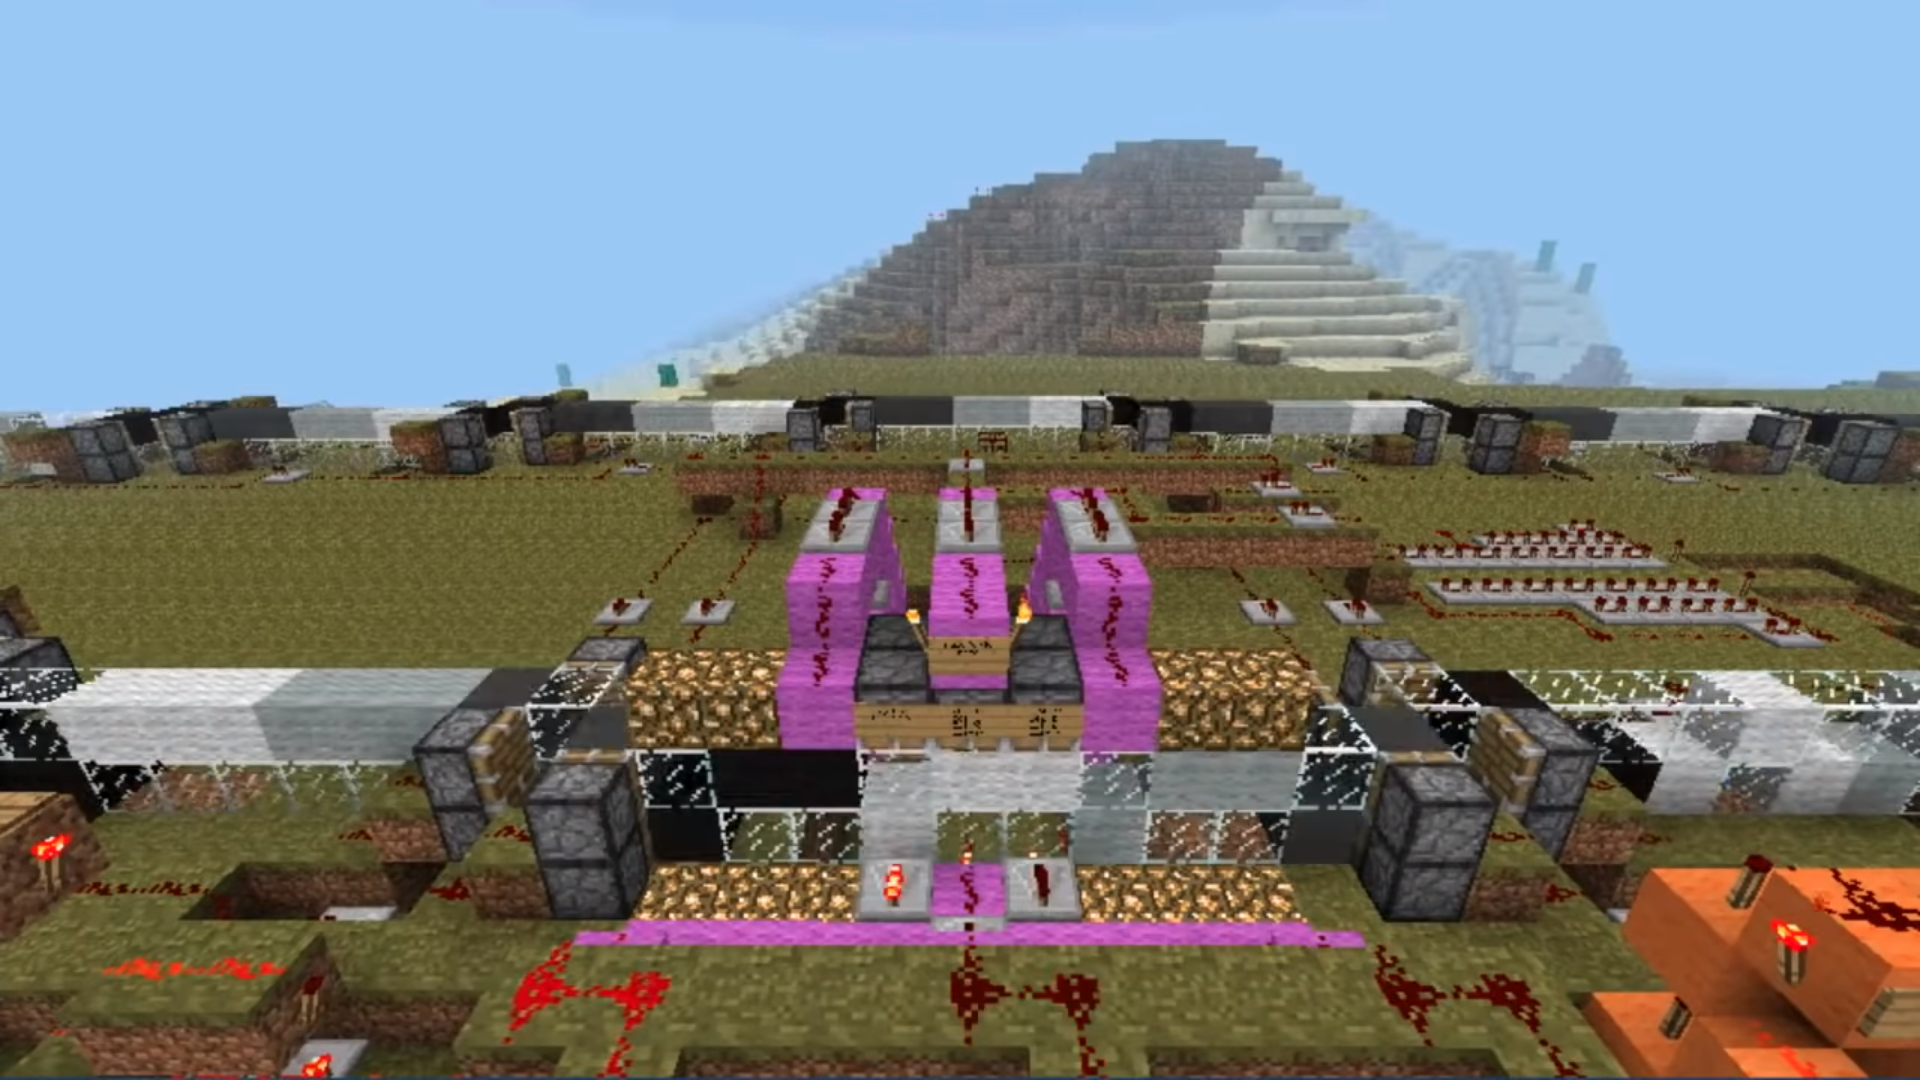
\includegraphics[height=2.2cm]{figures/turing_minecraft2.png}}
        \end{column}
    \end{columns}

    \begin{columns}
        \begin{column}{.6\hsize}
            {MS PowerPoint}
            {\footnotesize
            \begin{itemize}
                \myitem Tom Wildenhain, 2017 {\color{blue} \hyperlink{frame:przypisy}{(15)}}
                \myitem Wykorzystanie hiperłączy i animacji do zbudowania maszyny Turinga
            \end{itemize}
            }
        \end{column}
        \begin{column}{.45\hsize}
            {\hspace{0cm}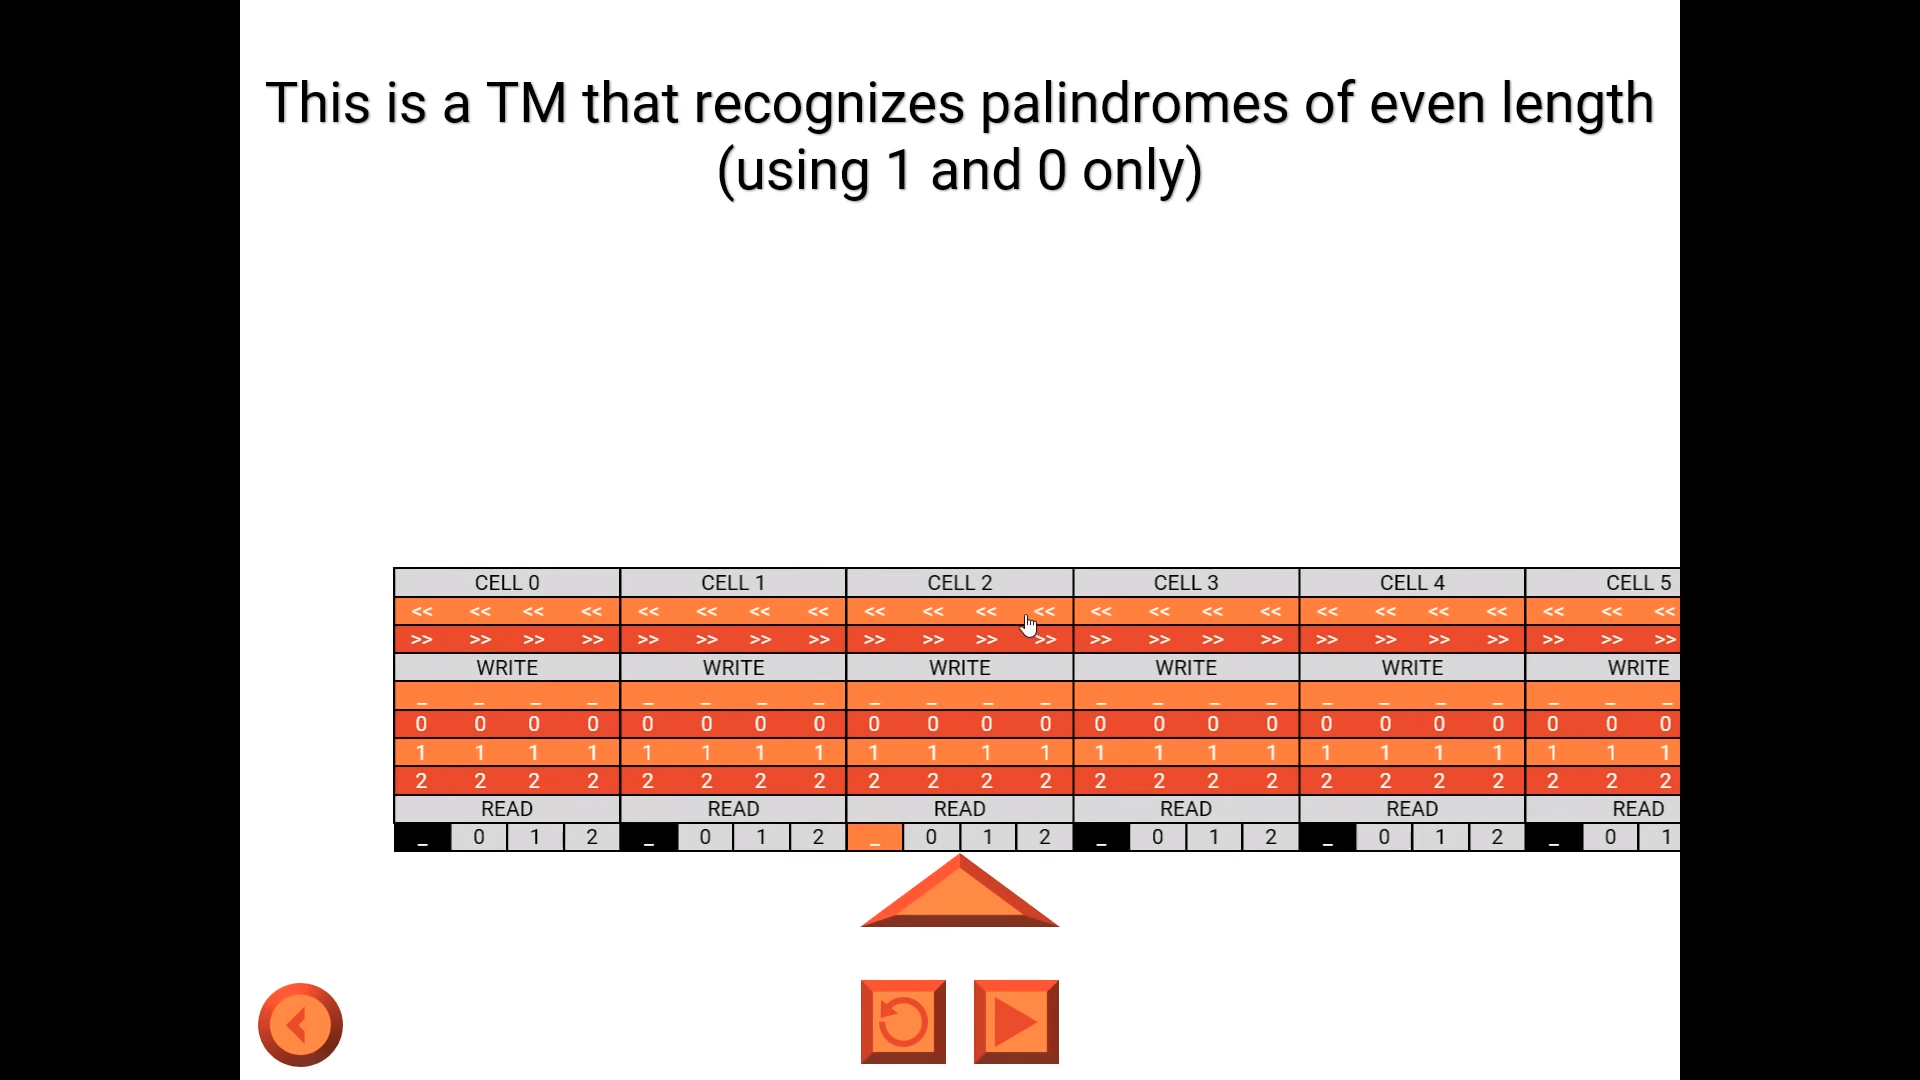
\includegraphics[height=2.2cm]{figures/turing_powerpoint.png}}
        \end{column}
    \end{columns}

    \begin{columns}
        \begin{column}{.6\hsize}
            {Magic the Gathering}
            {\footnotesize
            \begin{itemize}
                \myitem Alex Churchill, Stella Biderman, Austin Herrick, 2019 {\color{blue} \hyperlink{frame:przypisy}{(16)}}
                \myitem Statystyki niektórych kart przechowują informację o położeniu na taśmie maszyny Turinga (demonstracja autorstwa BecauseScience {\color{blue} \hyperlink{frame:przypisy}{(17)}})
            \end{itemize}
            }
        \end{column}
        \begin{column}{.45\hsize}
            {\hspace{0cm}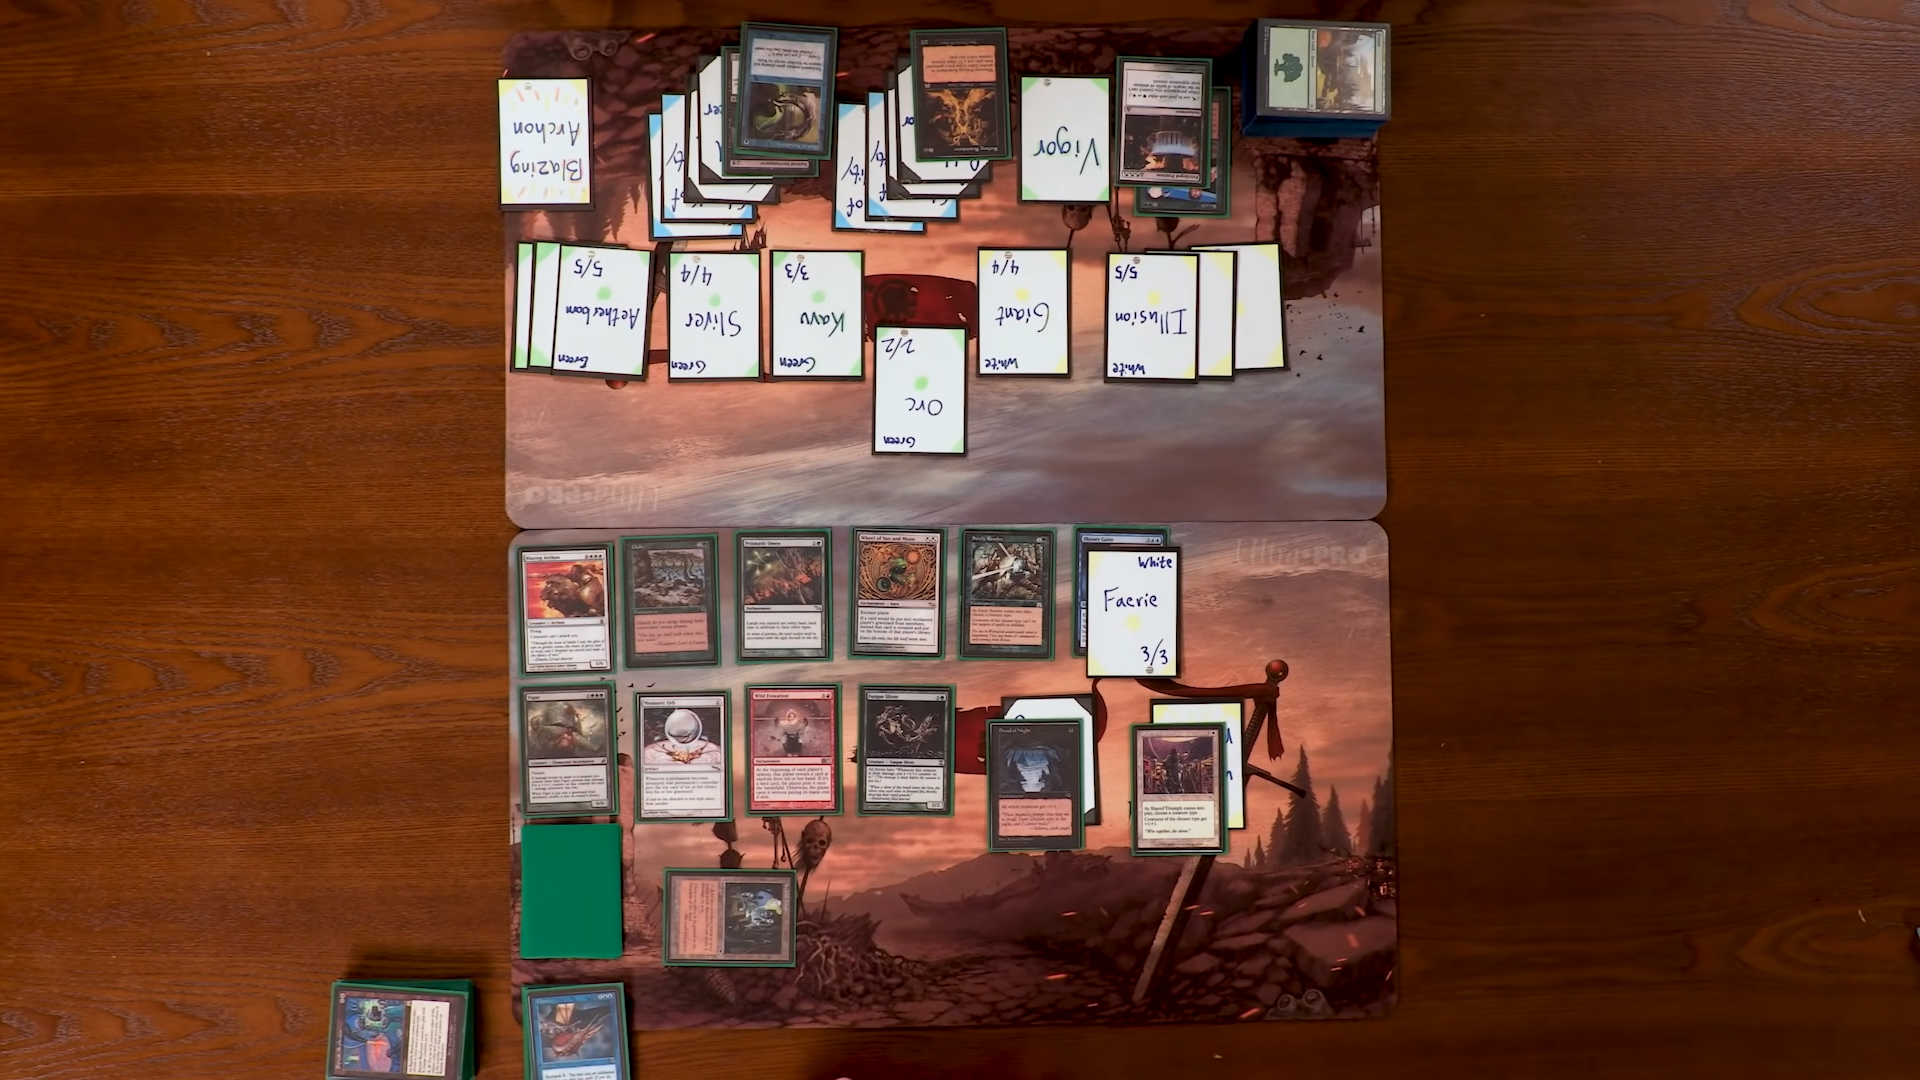
\includegraphics[height=2.2cm]{figures/turing_mtg.png}}
        \end{column}
    \end{columns}

\end{frame}
